\documentclass[fleqn,11pt]{article}

\usepackage[letterpaper,margin=0.75in]{geometry}

\usepackage{amsmath}
\usepackage{booktabs}
\usepackage{graphicx}
\usepackage{listings}

\setlength{\parindent}{1.4em}

\begin{document}

\lstset{
  language=Python,
  basicstyle=\small,          % print whole listing small
  keywordstyle=\bfseries,
  identifierstyle=,           % nothing happens
  commentstyle=,              % white comments
  stringstyle=\ttfamily,      % typewriter type for strings
  showstringspaces=false,     % no special string spaces
  numbers=left,
  numberstyle=\tiny,
  numbersep=5pt,
  frame=tb,
}

\title{Congestion Control Part 1}

\author{Spencer Wood}

\date{March 22, 2017}

\maketitle


I implemented TCP Tahoe congestion control inside a network simulator. I ran
several tests on the network dropping various amounts packets and compared them
to established data about how TCP congestion control works.\\
\indent In each test, a 515 KB pdf was transferred between two nodes in a two node
network with a bi-directional link. The bandwidth of the links was 1Mbps and
the latency was 100ms. The congestion window size and packet sequence activity
was recorded and graphed.\\


\section{Tests}

\subsection{Slow start}

\indent\indent This test involved transferring the PDF with no dropped packets. 

\begin{figure}[!htb]
  \centering
  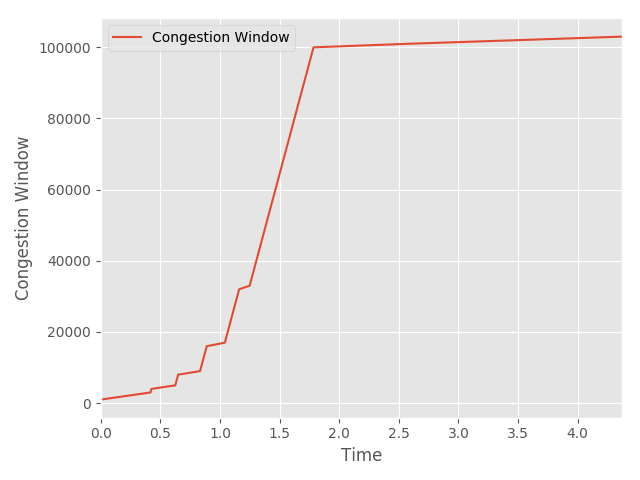
\includegraphics[width=8cm]{../graphs/0-cwnd.png}
  \caption{Congestion window for 0 dropped packets}
  \label{fig:throughput}
\end{figure}

Figures 1 shows the results of the test on the congestion window, and things
look as expected. Since there are no dropped packets, the congestion window
size grows rapidly until it reaches the threshold of 100,000, at which point it
grows linearly.

\newpage

\subsection{One packet loss}

\indent\indent This test involved transferring the PDF but dropping packet
14,000.

\begin{figure}[!htb]
  \centering
  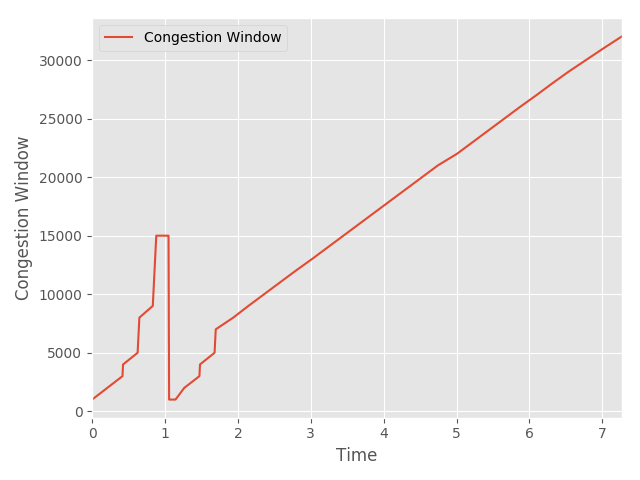
\includegraphics[width=8cm]{../graphs/1-cwnd.png}
  \caption{Congestion window for 1 dropped packet}
  \label{fig:throughput}
\end{figure}

\begin{figure}[!htb]
  \centering
  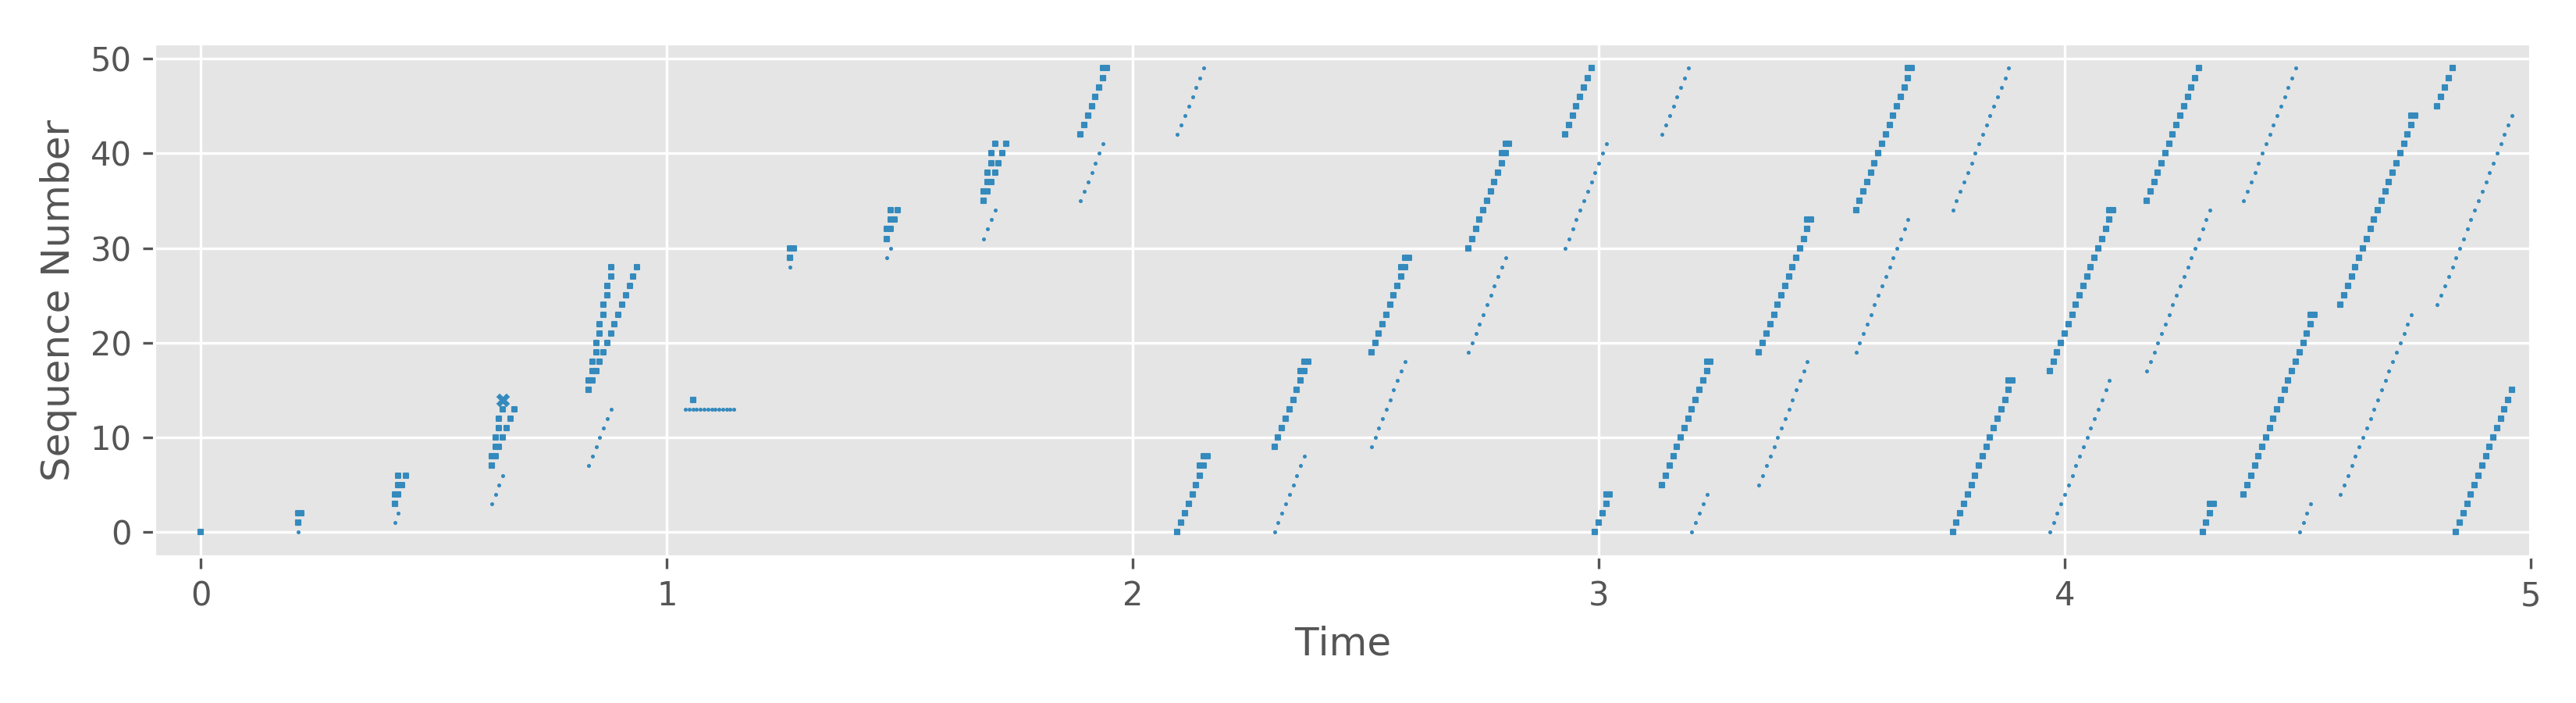
\includegraphics[width=13cm]{../graphs/1-sequence.png}
  \caption{Packet sequence events for 1 dropped packet}

  \label{fig:throughput}
\end{figure}

Figures 2 and 3 show the results of this test. The dropped packet is
represented by an X on the sequence graph. At the time the packet dropped there
was a dip in the congestion window as expected.

\newpage
\subsection{Two packet loss}

\indent\indent This test involved transferring the PDF but dropping packets
14,000 and 28,000. 

\begin{figure}[!htb]
  \centering
  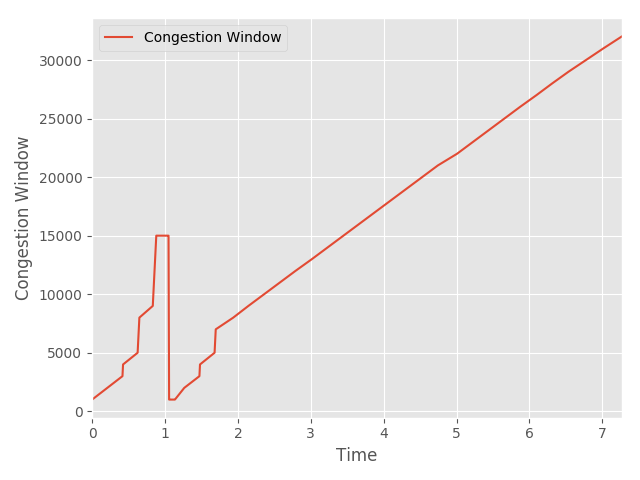
\includegraphics[width=8cm]{../graphs/2-cwnd.png}
  \caption{Congestion window for 2 dropped packets}
  \label{fig:throughput}
\end{figure}

\begin{figure}[!htb]
  \centering
  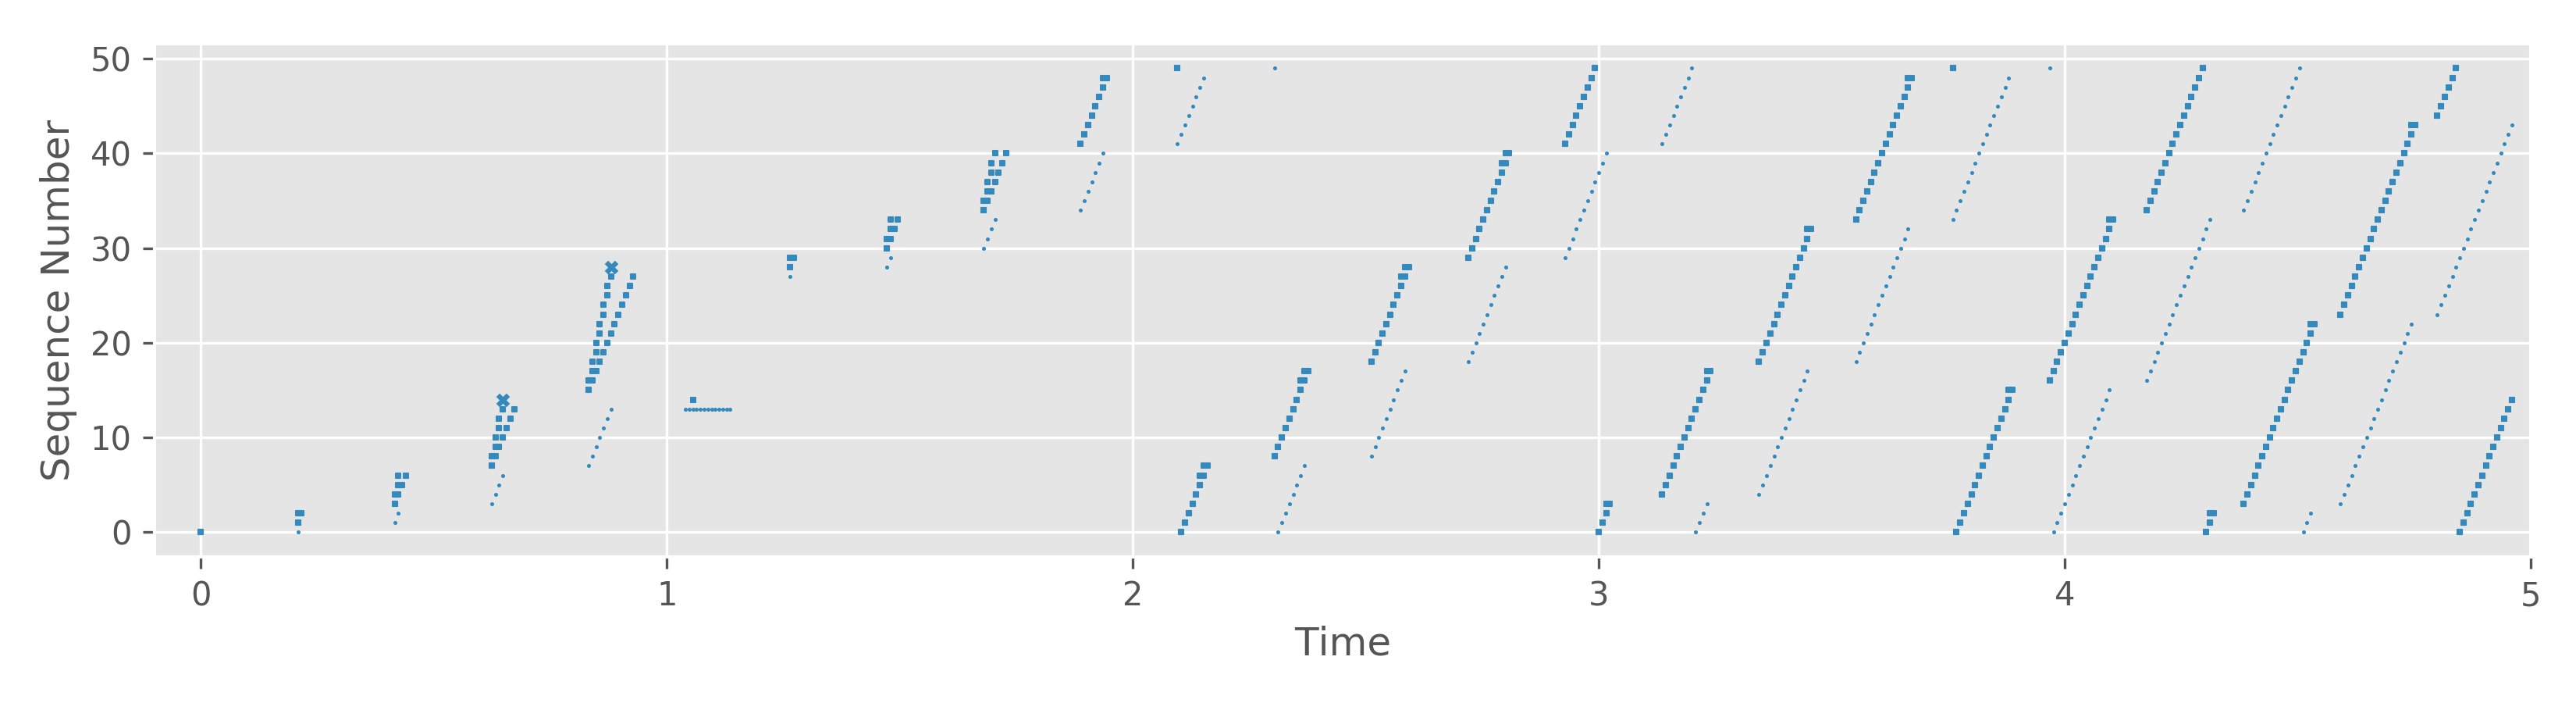
\includegraphics[width=13cm]{../graphs/2-sequence.png}
  \caption{Packet sequence events for 2 dropped packets}

  \label{fig:throughput}
\end{figure}

The results of this test came out as expected compared to the TCP SACK paper.

\newpage 
\subsection{Three packet loss}

\indent\indent This test involved transferring the PDF but dropping packets
14,000, 26,000, 28,000.

\begin{figure}[!htb]
  \centering
  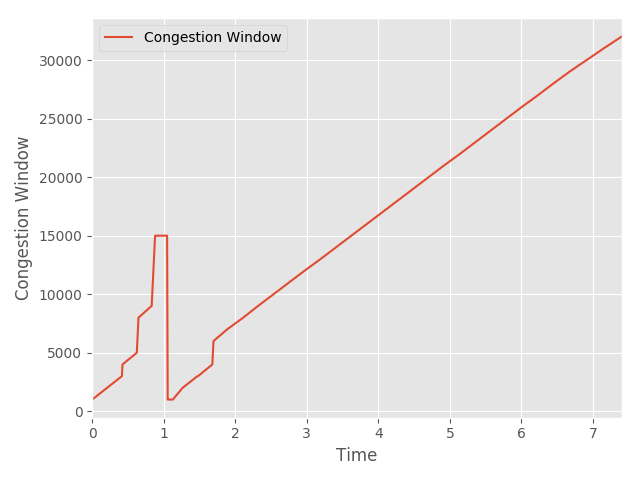
\includegraphics[width=8cm]{../graphs/3-cwnd.png}
  \caption{Congestion window for 3 dropped packets}
  \label{fig:throughput}
\end{figure}

\begin{figure}[!htb]
  \centering
  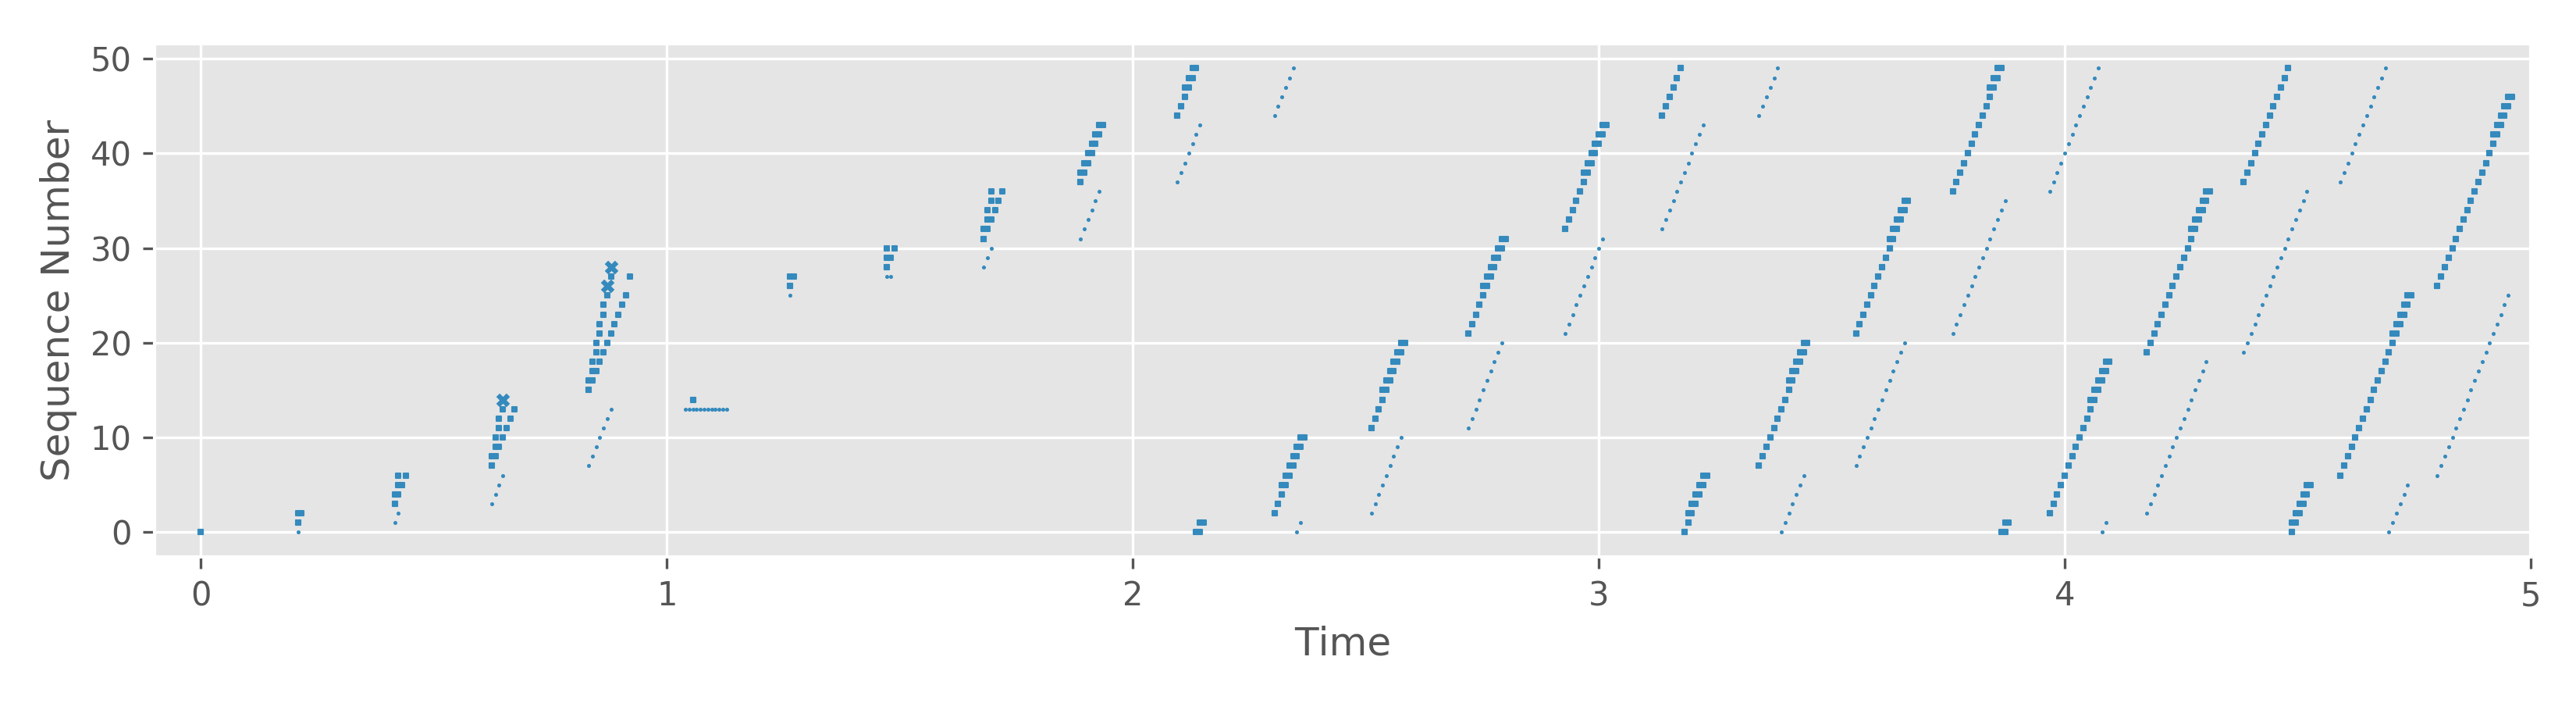
\includegraphics[width=13cm]{../graphs/3-sequence.png}
  \caption{Packet sequence events for 3 dropped packets}

  \label{fig:throughput}
\end{figure}

The results of this test came out as expected compared to the TCP SACK paper.

\end{document}
